% =============================================================================
% Chapter 8 — Speculative Decoding in Production: DSpark
% =============================================================================
\chapter{Speculative Decoding in Production: DSpark}
\label{ch:specdecode}

On a DGX Spark, a single decode step must stream roughly 16.5--17\,GB of
weights per rank out of LPDDR5X --- and that cost is almost independent of
how many tokens the step processes. Streaming the weights once to score seven
query rows costs nearly the same as streaming them to score one. Speculative
decoding is the mechanism that exploits this asymmetry, and everything this
recipe achieves at decode time flows through it. At the measured
$\approx$4.15 accepted tokens per step, the same hardware that would
otherwise deliver roughly 15 \tokspersec{} serves 62--83 \tokspersec{}
on TP=2 in the published August 2026 results --- which is why the
repository's audit methodology calls acceptance rate ``THE lever for decode
speed.'' (\Cref{ch:perf} records the lower September numbers, and the failed
search for what explains them.)

The lever has teeth. The drafter carries cross-step mutable state that vLLM's
scheduler knows nothing about, and it worked flawlessly single-stream ---
then, at \code{max_num_seqs > 1}, draft acceptance silently collapsed toward
zero with nothing crashing at all. This chapter teaches DSpark ---
DeepSeek-V4-Flash's built-in block drafter --- from the practitioner's side:
how the draft block is built, where the drafter hides its state, why that
state silently corrupted under concurrency and how three patches fixed it,
what acceptance actually looks like on live traffic (and how easily a bad
probe lies about it), how to choose the draft length $k$, and what tensor
parallelism does to the draft loop.

For an inference engineer, this is the chapter where the repository's model
knowledge, scheduler patches, and measurement discipline all meet: on
bandwidth-bound hardware, no other subsystem multiplies throughput the way
acceptance does, no other subsystem hides correctness bugs as quietly, and
no other metric is as easy to measure wrong.

\section{Why speculation pays on bandwidth-bound hardware}
\label{sec:specdecode-economics}

Autoregressive decode on a GB10 is a memory-bandwidth problem, not a compute
problem. The repository's first-principles accounting
(\Cref{sec:perf-costmodel} derives the full budget) puts one
TP=2 decode step for DeepSeek-V4-Flash at roughly 16.5--17\,GB of weight
traffic per rank --- about 12\,GB of routed experts, 2.4\,GB of attention
weights, 1.06\,GB of \code{lm_head}, plus the draft stack. At the
230--250\,GB/s effectively achievable on LPDDR5X, that traffic costs
68--74\,ms before any compute happens.

Speculative decoding exploits exactly the asymmetry the opening described. A
cheap drafter guesses the next $k$ tokens; the expensive target model then
runs \emph{one} forward pass over all $k{+}1$ positions (the $k$ drafts plus
the bonus token sampled at the first rejection point) and verifies them in
parallel. Every accepted draft token is a token produced without a dedicated
weight-streaming pass. At the acceptance the opening quoted, the bandwidth
bound alone predicts 56--61 \tokspersec{} against the August-published
62--83 band.
The analysis concludes that single-stream decode on TP=2 is
$\approx$80\,\% weight streaming, with the residual 10--15\,ms being fixed
software cost.

\begin{hbnote}
The break-even logic differs from datacenter GPUs. On compute-rich hardware,
speculative decoding must justify the drafter's FLOPs; on a GB10, drafter
compute is nearly free (the weights are small and the step is
bandwidth-idle), so the only question is acceptance. That is why this recipe
runs speculation always-on, and why every serving audit measures acceptance
before anything else.
\end{hbnote}

\section{The DSpark drafter}
\label{sec:specdecode-design}

The subsystem that must deliver that acceptance is DSpark --- which is not a
separate draft model. The checkpoint ships
\code{dspark_block_size=5} (the trained block width $\gamma$), a small stack of
draft layers in the historical \code{mtp.N.*} namespace, and a rank-256 Markov
head. The vLLM overlay (\repofile{recipe/overlay/vllm/models/deepseek_v4/nvidia/dspark.py},
$\approx$1{,}200 lines) turns these into a block drafter that rides vLLM's
EAGLE-family speculative plumbing under \code{method="dspark"}.

\subsection{One non-causal pass per block}

Stock MTP spends its draft layers on depth, looping one layer per drafted
token; DSpark spends them on width instead. Where stock DeepSeek MTP re-runs
its single MTP layer once per drafted token,
DSpark \emph{stacks} its draft stages into one non-causal backbone and predicts
the whole block in a single parallel pass. The drafter builds a
$[B, \gamma]$ query block per request: the \emph{anchor} token (the last
accepted token) first, then $\gamma{-}1$ trained \emph{noise} queries, at
positions $\mathrm{anchor} + [0, \gamma)$. The draft layers consume
concatenated target-layer features: the target model captures the
hyper-connection stream state after each layer in
\code{dspark_target_layer_ids}, collapses it, and writes it into a
stable-address buffer outside the cudagraph pool. The drafter therefore sees
rich mid-network features, not just the final hidden state.

Decoding the block is then \emph{left-to-right but cheap}: for each position
the base logits get a low-rank Markov bias,
\code{base_logits}\,${} + W_1[\mathrm{tok}]\,W_2^{\top}$ with both matrices
$129{,}280 \times 256$ (66\,MB each), conditioning position $i{+}1$ on the
token just chosen at position $i$. How the argmax over those biased logits
is computed, and whether drafts are sampled or taken greedily, are
implementation and configuration choices summarized in
\Cref{tab:specdecode-samplers}.

\begin{table}[htbp]
\centering\small
\caption{Draft sampling knobs. The three greedy implementations compute the
same argmax; \code{draft_sample_method} selects how drafts are drawn.}
\label{tab:specdecode-samplers}
\begin{tabular}{l>{\raggedright\arraybackslash}p{72mm}}
\toprule
Knob / mode & Behavior \\
\midrule
(default greedy path) & full-logits argmax over the biased logits \\
\envvar{VLLM_DSPARK_LOCAL_ARGMAX} & vocab-parallel local max with a gathered
  (value,\,index) reduction \\
\envvar{VLLM_DSPARK_FUSED_MARKOV_ARGMAX} & fused Triton kernel that never
  materializes the Markov logit vector \\
\code{draft_sample_method} & \code{probabilistic} (compose default; needs
  full draft logits for rejection sampling) or \code{greedy} (pairs with the
  official model cards' $k{=}7$ recommendation,
  \Cref{sec:specdecode-choosing-k}) \\
\bottomrule
\end{tabular}
\end{table}

\begin{figure}[htbp]
\centering
\begin{tikzpicture}[node distance=8mm and 5mm]
  % --- Draft phase ---
  \node[hbtitle] (t1) {1.\ Draft: one non-causal pass ($\gamma=5$)};
  \node[hbbox, below=4mm of t1, minimum width=22mm] (anchor) {anchor\\token};
  \node[hbnode, right=3mm of anchor, minimum width=34mm] (noise) {noise queries\\$q_1 \dots q_4$};
  \node[hbnode, right=3mm of noise, minimum width=34mm] (markov) {Markov head\\left-to-right};
  \node[hbgpu, right=3mm of markov, minimum width=26mm] (draft) {drafts\\$d_1 \dots d_5$};
  \draw[hbflow] (anchor) -- (noise);
  \draw[hbflow] (noise) -- (markov);
  \draw[hbflow] (markov) -- (draft);
  % --- Verify phase ---
  \node[hbtitle, below=14mm of anchor.south west, anchor=west] (t2)
    {2.\ Verify: one target pass over $k{+}1$ rows};
  \node[hbbox, below=4mm of t2.south west, anchor=north west, minimum width=96mm]
    (verify) {target forward: $[\,t,\ d_1,\ d_2,\ d_3,\ d_4,\ d_5\,]$ --- weights streamed \textbf{once}};
  \draw[hbflow] (draft.south) to[out=-90,in=30] (verify.east);
  % --- Accept phase ---
  \node[hbtitle, below=6mm of verify.south west, anchor=north west] (t3)
    {3.\ Rejection sampling};
  \node[hbgpu, below=4mm of t3.south west, anchor=north west, minimum width=13mm] (a1) {$d_1$ \checkmark};
  \node[hbgpu, right=2.5mm of a1, minimum width=13mm] (a2) {$d_2$ \checkmark};
  \node[hbgpu, right=2.5mm of a2, minimum width=13mm] (a3) {$d_3$ \checkmark};
  \node[hbwarn, right=2.5mm of a3, minimum width=13mm] (r1) {$d_4$ $\times$};
  \node[hbfaint, right=2.5mm of r1, minimum width=13mm] (r2) {$d_5$};
  \node[hbbox, right=6mm of r2, minimum width=24mm] (bonus) {bonus token\\(target)};
  \draw[hbok] (verify.south -| a3) to[out=-90,in=90] (a3.north);
  \draw[hbarrow] (r1.north) to[out=60,in=120,looseness=0.9] (bonus.north);
  \node[hblabel, below=2mm of a2.south east] {accepted prefix kept: 3 drafts $+$ 1 bonus $=$ 4 tokens this step};
\end{tikzpicture}
\caption{One DSpark decode step. The drafter predicts a whole
$\gamma$-token block in a single non-causal pass (anchor plus noise
queries), samples it left-to-right through the rank-256 Markov head, and the
target verifies all $k{+}1$ positions in one forward pass. The accepted
prefix survives; the first rejection yields the target's own bonus token and
discards the rest.}
\label{fig:specdecode-timeline}
\end{figure}

\subsection{Private state: ring buffers outside the paged KV}

The design decision that dominates the rest of this chapter: the drafter's KV
is \emph{not} vLLM KV cache. \code{DSparkProposer.initialize_attn_backend} is
a no-op (\code{block_size = 1}, no KV layers registered). Instead, each draft
attention module owns a persistent tensor
\code{main_kv_cache[max_num_seqs, window, head_dim]} --- a per-request sliding
window of projected target features, written as a ring buffer
(\texttt{position \% window}) --- plus a scratch buffer for sparse attention
scores. Draft attention runs over
\code{[main-window | draft-block]} with an attention-sink term in the softmax
normalizer. This sidesteps the paged-KV allocator entirely
(\Cref{fig:specdecode-kv-layout}), but it also means
the drafter carries cross-step mutable state that vLLM's scheduler knows
nothing about. That is a loaded gun, and \Cref{sec:specdecode-keys} is the
story of it going off.

\begin{figure}[htbp]
\centering
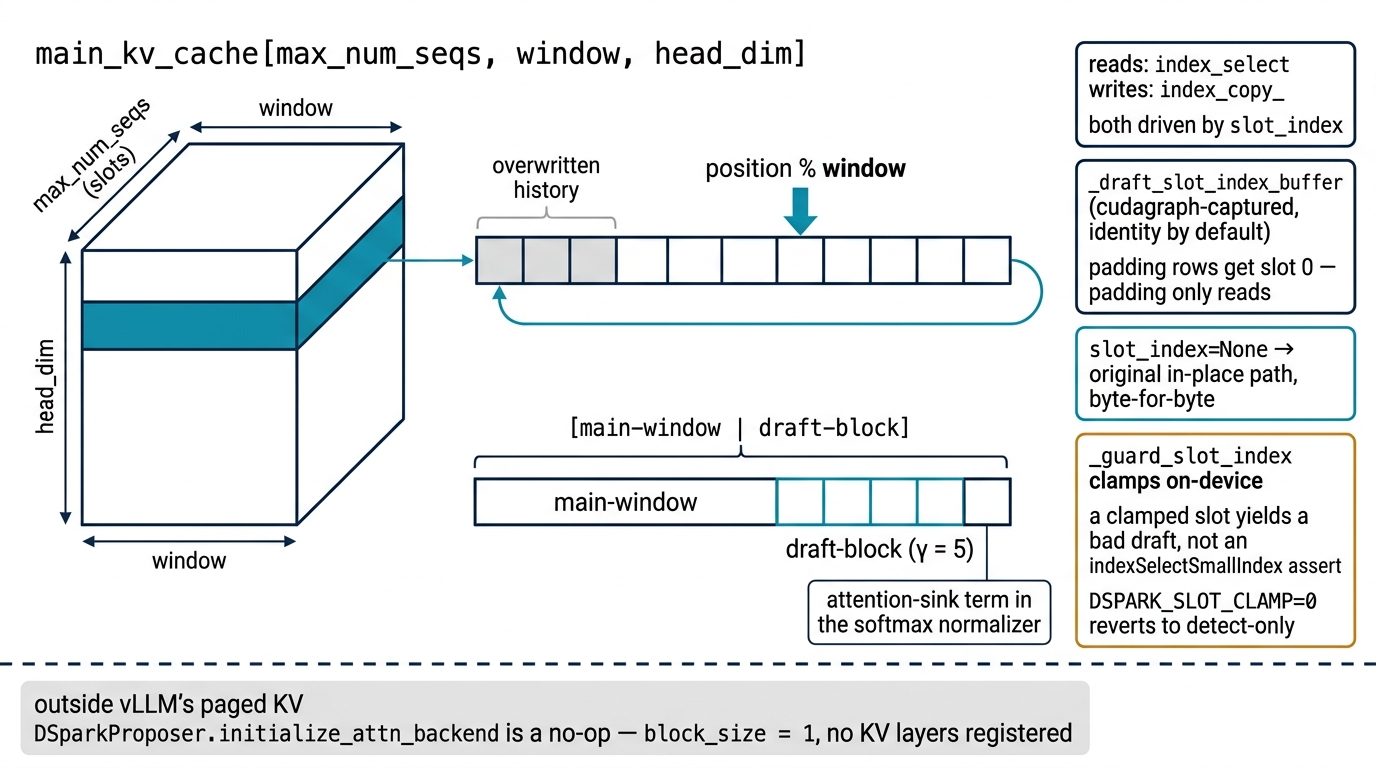
\includegraphics[width=\textwidth]{figures/ch08-drafter-kv-layout.png}
\caption{The drafter's only cross-step state. Each draft attention module
owns a persistent \code{main_kv_cache[max_num_seqs, window, head_dim]} --- a
per-request sliding window of projected target features written as a ring at
\texttt{position \% window} --- and draft attention runs over
\code{[main-window | draft-block]} with an attention-sink term in the softmax
normalizer. \code{initialize_attn_backend} is a no-op
(\code{block_size = 1}, no KV layers registered), so this sidesteps the
paged-KV allocator entirely. Reads gather and writes scatter through
\code{slot_index}; when the permutation is the identity the proposer passes
\code{slot_index=None} and the original in-place path runs byte-for-byte.}
\label{fig:specdecode-kv-layout}
\end{figure}

\section{The concurrency correctness saga}
\label{sec:specdecode-keys}

Single-stream, DSpark worked from day one. Turning up
\code{max_num_seqs} produced two distinct failures --- one silent, one loud
--- fixed by the ``Keys'' patch series
(\repofile{patches/keys-concurrency.patch}, documented as Patch~1, Patch~2,
and Patch~2b in \repofile{docs/PATCHES.md}). Together they are the best
worked example in the repository of a stateful component meeting a batch-condensing
scheduler.

\subsection{Patch 1: batch rows are not identities}

\textbf{Symptom.} At \code{max_num_seqs > 1}, draft acceptance collapsed
toward zero. Nothing crashed; the engine silently degraded to
verify-everything-reject-everything throughput.

\textbf{Root cause.} The ring buffers were indexed by \emph{batch-row
position} (\code{main_kv_cache[:batch_size]}), and the proposer carried no
request identity. vLLM v1's continuous batching \emph{condenses} the running
batch whenever a request finishes: a later request is moved into the freed
row. The model-side ring buffer row is not moved with it. After a condense,
a request reads a sliding-window history that belongs to a \emph{different}
request --- corrupted draft context, garbage drafts, acceptance collapse.
Single-stream never condenses row~0, which is exactly why the bug hid.

\textbf{Fix.} Key the state by a stable per-request slot. The proposer keeps
\code{_req_id_to_slot} and a free-slot pool: \code{_row_to_slot(req_ids)}
reclaims slots of finished requests, assigns free slots lowest-first, and
returns slots in batch-row order. The model runner threads
\code{req_ids=self.input_batch.req_ids} into \code{propose()} (a kwarg only
the DSpark proposer accepts). On the model side, \code{store_main_kv} and the
draft forward accept a \code{slot_index}: reads gather with
\code{index_select}, writes scatter with \code{index_copy_}, so the ring
follows the request id, not the row. A persistent cudagraph-captured
\code{_draft_slot_index_buffer} (identity by default) carries the slots into
the graphed draft path; padding rows get slot~0, which is safe because
padding only reads.

The elegant part is the escape hatch: when the resolved permutation is the
identity --- which a genuine single-request server always produces, since
lowest-first assignment keeps it on slot~0 --- the proposer passes
\code{slot_index=None} and the original in-place code path runs
\emph{byte-for-byte}. Warmup, capture, and single-stream serving are
provably unchanged. Gating on permutation identity rather than on
\code{batch == 1} also keeps the ``batch condensed down to one surviving
request holding a non-zero slot'' case correct.

One rule survives this whole chapter intact, and Patch~1 is where it is
written down: any state that outlives a single step must be keyed by a stable
request identity, never by a position in a batch the scheduler is free to
rearrange. The drafter's ring buffers broke that rule and degraded silently;
nothing crashed, and only acceptance recorded the damage.

\begin{figure}[htbp]
\centering
\begin{tikzpicture}[node distance=6mm and 8mm]
  % ---- LEFT: broken ----
  \node[hbtitle] (lt) {Batch-row indexing (broken)};
  \node[hbnode, below=4mm of lt, minimum width=30mm] (l0) {batch row 0: req A};
  \node[hbnode, below=3mm of l0, minimum width=30mm] (l1) {batch row 1: req B};
  \node[hbwarn, below=8mm of l1, minimum width=30mm] (lc0) {row 0: \textbf{req B}};
  \node[hblabel, align=left, right=2mm of l1.east, anchor=west] {A finishes,\\batch condenses};
  \draw[hbfail] (l1.south) -- (lc0.north);
  % ring buffers
  \node[hbhost, below=8mm of lc0, minimum width=30mm] (lr0) {ring 0: A's KV};
  \node[hbhost, below=3mm of lr0, minimum width=30mm] (lr1) {ring 1: B's KV};
  \draw[hbfail] (lc0.south) -- node[hblabel, left=1mm] {reads row 0} (lr0.north);
  \node[hblabel, below=2mm of lr1] {B drafts from A's history $\rightarrow$ acceptance $\rightarrow$ 0};
  % ---- RIGHT: fixed ----
  \node[hbtitle, right=42mm of lt] (rt) {Slot indexing (Patch 1)};
  \node[hbnode, below=4mm of rt, minimum width=34mm] (m0) {req A $\rightarrow$ slot 0};
  \node[hbnode, below=3mm of m0, minimum width=34mm] (m1) {req B $\rightarrow$ slot 1};
  \node[hbgpu, below=8mm of m1, minimum width=34mm] (rc0) {row 0: req B};
  \node[hblabel, align=left, right=2mm of m1.east, anchor=west] {condense;\\slots stable};
  \draw[hbok] (m1.south) -- (rc0.north);
  \node[hbhost, below=8mm of rc0, minimum width=34mm] (rr0) {ring 0: A's KV (freed)};
  \node[hbhost, below=3mm of rr0, minimum width=34mm] (rr1) {ring 1: B's KV};
  \draw[hbok] (rc0.east) to[out=-15,in=25]
    node[hblabel, pos=0.5, anchor=west, xshift=0.5mm, align=left, font=\tiny]
    {slot\_index\\gather} (rr1.east);
  \node[hblabel, below=2mm of rr1] {B always reads slot 1, wherever its row lands};
\end{tikzpicture}
\caption{Why acceptance collapsed under concurrency. Left: vLLM v1 condenses
the batch when request A finishes, moving request B to row 0 --- but the
drafter's persistent ring buffer stays put, so B drafts from A's
sliding-window history. Right: Patch 1 keys the ring by a stable per-request
slot; reads gather through \texttt{slot\_index}, and an identity permutation
falls back to the original in-place path byte-for-byte.}
\label{fig:specdecode-slots}
\end{figure}

\subsection{Patch 2: chunked prefill makes batches ragged}

\textbf{Symptom.} With slots fixed, realistic staggered arrivals produced
HTTP~500s:

\begin{lstlisting}
ValueError: DSpark currently requires uniform flattened per-request inputs;
got 41 rows for batch_size=2.   (dspark_proposer.py: _view_by_request)
\end{lstlisting}

\textbf{Root cause.} \code{prepare_context} reshaped the flat target hidden
states into a rectangular \code{[batch, seq, H]} view, asserting equal row
counts per request. With chunked prefill --- mandatory at long context, since
disabling it requires \code{max_num_batched_tokens >= max_model_len} --- a
single step mixes prefill and decode rows (``41 rows for batch\_size=2'' is
one request prefilling next to one decoding). The static benchmark had
passed only because all its prompts were identical length.

\textbf{Fix.} A ragged path keyed on \code{query_start_loc}: detect
non-uniform segment lengths, skip the rectangular view, compute each
request's draft anchor with a flat index
(\texttt{starts + clamp(len - rejected - 1, 0, len-1)}) and
\code{index_select} the per-request last hidden state. Storage never needed
uniformity in the first place --- it is position-addressed
(\texttt{position \% window}). A new \code{_store_main_kv_ragged} therefore
segments the flat rows, trims each segment to the window, applies the
rejected-suffix mask, and \code{index_copy_}s into each request's slot ring.
Ragged steps run eager, which is safe because mixed prefill/decode steps are
never cudagraph-captured; the uniform decode-only graphed path is untouched.
Only the \envvar{VLLM_DSPARK_GPU_REJECTED_CONTEXT_MASK=1} path was made
ragged, so serving must run with that flag set.

\subsection{Patch 2b: raggedness is not rejection}

A GSM8K quality eval --- not a benchmark --- found the last crack. A
prefill-heavy step with \emph{no} rejected tokens still crashed
(\code{got 166 rows for batch_size=3}): Patch~2 had computed \code{ragged}
only inside the branch where \code{num_rejected_tokens_gpu is not None},
but raggedness depends on \code{query_start_loc} segment lengths, not on
rejection. Fresh requests prefilling together, with nothing to reject, fell
through to the rectangular view. Patch~2b enters ragged detection whenever
the GPU-mask mode is on, regardless of the rejection tensor, defaulting
\code{rejected} to zeros when absent (\Cref{fig:specdecode-ragged-views}).
Earlier staggered tests had missed it
because their prompts were uniform-ish; GSM8K's varied prompt lengths hit it
immediately. The re-run after the fix: 200 questions at $N{=}8$ concurrency,
0 errors, 93.5\,\% accuracy vs.\ 95.0\,\% sequential, 97.5\,\% per-question
agreement --- quality-neutral within batch floating-point nondeterminism.

\begin{figure}[htbp]
\centering
\adjustbox{max width=\textwidth}{%
\begin{tikzpicture}[font=\scriptsize]
  % =================== PANEL 1 ===================
  \node[hbtitle, anchor=north west] at (0,13.90)
    {\#1 --- got 41 rows for \texttt{batch\_size=2}};

  \node[hblabel, anchor=south west, color=navy] at (0,12.92) {\texttt{query\_start\_loc}};
  \node[hblabel, anchor=south, color=navy] at (9.31,12.92) {decode};
  % flat strip of 41 rows: 40 prefill + 1 decode
  \foreach \i in {0,...,39} {
    \fill[teal!18] ({0.23*\i},12.15) rectangle ({0.23*\i+0.23},12.70);
    \draw[lightgray] ({0.23*\i},12.15) -- ({0.23*\i},12.70);
  }
  \fill[brandcyan!40] (9.20,12.15) rectangle (9.43,12.70);
  \draw[navy, thick] (0,12.15) rectangle (9.43,12.70);
  \foreach \x in {0,9.20,9.43} { \draw[navy, line width=1.1pt] (\x,12.03) -- (\x,12.82); }
  \node[anchor=center, font=\scriptsize, color=navy] at (4.60,12.425) {prefill};

  % ghosted rectangular view whose gridlines do not tile the strip
  \draw[brandgray!80, dashed] (0,11.30) rectangle (9.43,11.85);
  \draw[brandgray!80, dashed] (4.715,11.30) -- (4.715,11.85);
  \draw[clueerror!80, dashed, line width=0.8pt] (4.715,11.86) -- (4.715,12.14);
  \node[anchor=center, font=\scriptsize, color=brandgray] at (2.36,11.575)
    {\texttt{[batch, seq, H]}};

  \node[hbwarn, anchor=west, align=left, font=\scriptsize, text width=4.9cm]
        (err) at (10.40,12.10)
    {\texttt{ValueError: DSpark currently requires uniform flattened
      per-request inputs}\\[2pt]
     \texttt{dspark\_proposer.py: \_view\_by\_request}};
  \draw[hbfail] (9.55,12.42) to[out=0,in=170] (err.west);

  \node[hbfaint, anchor=north west, align=left, font=\scriptsize, text width=9.2cm,
        minimum height=0mm, inner sep=4pt] at (0,11.05)
    {the static benchmark passed --- all its prompts were the same length};

  \draw[lightgray] (0,10.30) -- (15.8,10.30);

  % =================== PANEL 2 ===================
  \node[hbtitle, anchor=north west] at (0,10.10)
    {\#2 --- got 166 rows for \texttt{batch\_size=3}};

  \draw[brandgray, thick] (0,9.00) rectangle (9.43,9.35);
  \node[hblabel, anchor=west] at (9.62,9.175) {rejection tensor: all zeros};

  % three unequal prefill segments
  \fill[teal!18] (0,8.30) rectangle (9.43,8.85);
  \draw[navy, thick] (0,8.30) rectangle (9.43,8.85);
  \foreach \x in {0,3.60,6.20,9.43} { \draw[navy, line width=1.1pt] (\x,8.18) -- (\x,8.97); }
  \node[hblabel, anchor=west, color=navy] at (9.62,8.575) {\texttt{query\_start\_loc}};

  \node[hbwarn, anchor=north west, align=left, font=\scriptsize, text width=6.0cm]
        (gate2) at (0,7.90)
    {Patch 2 computed \texttt{ragged} only inside
     \texttt{num\_rejected\_tokens\_gpu is not None}};
  \draw[hbfail] (1.80,8.16) -- (1.80,7.96);

  \draw[brandgray!80, dashed] (11.60,7.10) rectangle (15.70,7.65);
  \draw[brandgray!80, dashed] (12.97,7.10) -- (12.97,7.65);
  \draw[brandgray!80, dashed] (14.34,7.10) -- (14.34,7.65);
  \node[anchor=south, font=\scriptsize, color=brandgray] at (13.65,7.74)
    {\texttt{[batch, seq, H]}};
  \draw[hbfail] (6.42,7.40) -- (11.50,7.40);
  \node[hblabel, anchor=north west, color=clueerror] at (6.55,7.26)
    {routed back to the rectangular view};

  \node[anchor=north west, font=\scriptsize\bfseries, color=teal] at (0,6.72)
    {raggedness depends on segment lengths, not on rejection};

  \draw[lightgray] (0,6.15) -- (15.8,6.15);

  % =================== PANEL 3 ===================
  \node[hbtitle, anchor=south west, color=brandgreen!60!black] at (0,5.70) {fixed path};
  \draw[brandgreen!70!black, dashed, rounded corners=4pt] (-0.25,3.70) rectangle (15.45,5.60);

  \node[hbgpu, anchor=north west, align=left, font=\scriptsize,
        text width=2.70cm, minimum height=14mm] (s1) at (0,5.28)
    {detect non-uniform lengths from \texttt{query\_start\_loc}};
  \node[hbgpu, anchor=north west, align=left, font=\scriptsize,
        text width=2.70cm, minimum height=14mm] (s2) at (3.60,5.28)
    {\texttt{starts + clamp(len - rejected - 1, 0, len-1)}};
  \node[hbgpu, anchor=north west, align=left, font=\scriptsize,
        text width=2.70cm, minimum height=14mm] (s3) at (7.20,5.28)
    {\texttt{index\_select} the per-request last hidden state};
  \node[hbgpu, anchor=north west, align=left, font=\scriptsize,
        text width=4.60cm, minimum height=14mm] (s4) at (10.80,5.28)
    {\texttt{\_store\_main\_kv\_ragged} $\rightarrow$ trim to window
     $\rightarrow$ \texttt{index\_copy\_} into each slot ring};
  \draw[hbok] (3.12,4.58) -- (3.55,4.58);
  \draw[hbok] (6.72,4.58) -- (7.15,4.58);
  \draw[hbok] (10.32,4.58) -- (10.75,4.58);

  % =================== badges ===================
  \node[hbpatch, anchor=north west, align=left, font=\scriptsize, text width=6.6cm]
        at (0,3.30)
    {ragged steps run eager --- mixed prefill/decode steps are never
     cudagraph-captured};
  \node[hbnode, draw=navy, anchor=north west, align=left, font=\scriptsize,
        text width=7.4cm] at (7.60,3.30)
    {\texttt{VLLM\_DSPARK\_GPU\_REJECTED\_CONTEXT\_MASK=1} required};
  \node[hbgpu, anchor=north west, align=left, font=\scriptsize, text width=14.8cm]
        at (0,2.20)
    {found by GSM8K, not a benchmark --- 200 questions at N=8, 0 errors,
     93.5\,\% vs 95.0\,\%, 97.5\,\% agreement};
\end{tikzpicture}%
}
\caption{Patches 2 and 2b. \code{prepare_context} reshaped the flat target
hidden states into a rectangular \code{[batch, seq, H]} view asserting equal
rows per request, but chunked prefill mixes a prefilling request beside a
decoding one in the same step --- \code{got 41 rows for batch_size=2}.
Patch~2 added a ragged path keyed on \code{query_start_loc} but computed
raggedness only inside the branch where a rejection tensor existed, so three
fresh requests prefilling together with nothing to reject still fell through
to the rectangular view --- \code{got 166 rows for batch_size=3}. Patch~2b
decoupled the two: ragged detection runs whenever GPU-mask mode is on, with
\code{rejected} defaulting to zeros. Found by a GSM8K quality eval, not a
benchmark.}
\label{fig:specdecode-ragged-views}
\end{figure}

\begin{hbwarstory}
Before the slot map, the failure mode at long context was worse than bad
drafts: a stale row index after condensation could fire a device-side
\code{indexSelectSmallIndex} assert and kill the whole WorkerProc. The
overlay's \code{_guard_slot_index} now clamps out-of-range slots on-device
(graph-safe) and logs loudly on eager paths --- a clamped slot merely yields
a bad draft that the target rejects, instead of a dead engine. The kill
switch \envvar{DSPARK_SLOT_CLAMP=0} reverts to detect-only for A/B. The same
defensive spirit shows in the proposer's non-uniform batch guard: flattened
rows that do not divide evenly by the batch produce a one-time warning and a
skipped speculation step, never a crash.
\end{hbwarstory}

\subsection{Reproducing it: the A/B replica protocol}

\repofile{docs/SETUP.md} encodes the validation discipline: two independent
TP=2 replicas on the four Sparks, serving the \emph{same}
DeepSeek-V4-Flash-DSpark weights. Replica~A (the Rafael Caricio stack) is
the unpatched control pinned at \code{max-num-seqs=1}; replica~B (the
TonyD2Wild packaged recipe) carries the patch and sweeps
\code{max-num-seqs} 1$\to$16. Both idle at $\approx$52--54 \tokspersec{}
single-stream, so any concurrency difference is attributable to the patch,
not the packaging. The reproduction is four steps:

\begin{lstlisting}[language=bash]
git apply -p1 patches/keys-concurrency.patch   # in the overlay checkout
./build-dspark-vllm-runtime.sh                 # rebuild on every node
# .env:
#   MAX_NUM_SEQS=16
#   VLLM_DSPARK_GPU_REJECTED_CONTEXT_MASK=1    # required for the ragged path
./smoke-deepseek-v4-flash-dspark.sh            # after worker-first restart
\end{lstlisting}

\section{Acceptance in practice}
\label{sec:specdecode-acceptance}

With the drafter correct under concurrency, the question returns to the one
that justifies its existence: how much of what it drafts survives
verification --- and how to measure that without fooling yourself.

\subsection{The shape of the curve}

Per-position acceptance is the honest fingerprint of a drafter. On this
recipe the audit's expected healthy curve (\repofile{scripts/EVAL.md} and
\repofile{AUDIT.md}, verified 2026-08-16) runs from pos0
$\approx$0.93 down to pos4 $\approx$0.33 --- the ``normal DSpark collapse.''
A live TP=3 probe put concrete deltas behind it: over one measurement window,
2{,}004 accepted of 4{,}140 drafted tokens = \textbf{48.4\,\%} overall, with
the per-position curve 0.92 / 0.74 / 0.60 / 0.41 / 0.28 / 0.21. The
tokens-per-step arithmetic is worth internalizing: 4{,}140 draft tokens at
$k{=}6$ means 690 draft rounds; $2004/690 \approx 2.9$ accepted per round;
plus the guaranteed verified target token, $\approx$\textbf{3.9 tokens per
step}. That single number, multiplied by the step rate, \emph{is} the decode
throughput.

\Cref{fig:specdecode-curve} shows the $k{=}5$-vs-$k{=}6$ comparison measured
for the block-$k$ work (\Cref{sec:specdecode-choosing-k}): the 0731
checkpoint at its trained $k{=}5$ holds up much better in the tail
(pos4 0.47 vs.\ 0.23), and $k{=}6$'s sixth position accepts only 0.15 ---
drafting it costs more step time than it returns.

\subsection{Acceptance is prompt-dependent --- and probes lie}

The single most operationally important fact: acceptance on this draft head
varies enormously with the prompt (\Cref{fig:specdecode-probe-families}).
The audit-style numbered-word probes sit
at pos0 $\ge 0.90$ with a healthy curve; \emph{live natural-prose} traffic
measured pos0 0.66--0.71 and $\approx$25\,\% overall acceptance, with the
cumulative live counter around 0.78. During the September A/B campaign this
gap nearly derailed a diagnosis: a recovery gate demanded pos0 $\ge 0.85$,
and the live lane showed 0.68. Only tracing the bar back to the audit
report's ``good prompts'' curve established that 0.66--0.71 was a
pre-existing live-vs-audit gap, not a regression. The vision lane's
Prometheus snapshot tells the same story in miniature: 23.7\,\% acceptance
with positions 2--5 nearly dead (per-position accepted counts
84/63/1/1/0/0) --- natural-prose drafting, not a broken engine.

\begin{figure}[htbp]
\centering
\begin{tikzpicture}[x=1cm,y=45mm]
  % axes and gridlines
  \foreach \y/\l in {0.2/0.2, 0.4/0.4, 0.6/0.6, 0.8/0.8, 1.0/1.0} {
    \draw[hbSteel!25] (0,\y) -- (12.4,\y);
    \node[hblabel, left=1mm] at (0,\y) {\l};
  }
  \draw[thick, hbSteel] (0,0) -- (12.4,0);
  \draw[thick, hbSteel] (0,0) -- (0,1.05);
  % bars: k=5 (green), k=6 (blue); group origin 0.7 + p*2
  \foreach \p/\vfive in {0/0.93, 1/0.75, 2/0.66, 3/0.58, 4/0.47} {
    \fill[hbGreen!60] ({0.7+\p*2},0) rectangle ({1.3+\p*2},\vfive);
    \node[hblabel] at ({1.0+\p*2},{\vfive+0.045}) {\vfive};
  }
  \foreach \p/\vsix in {0/0.89, 1/0.73, 2/0.49, 3/0.34, 4/0.23, 5/0.15} {
    \fill[hbBlue!60] ({1.4+\p*2},0) rectangle ({2.0+\p*2},\vsix);
    \node[hblabel] at ({1.7+\p*2},{\vsix+0.045}) {\vsix};
  }
  % x labels
  \foreach \p in {0,1,2,3,4,5} {
    \node[hblabel] at ({1.35+\p*2},-0.06) {pos \p};
  }
  % legend
  \fill[hbGreen!60] (8.6,0.93) rectangle (9.0,0.99);
  \node[hblabel, right=1mm, anchor=west] at (9.0,0.96) {0731, $k{=}5$ (trained block)};
  \fill[hbBlue!60] (8.6,0.82) rectangle (9.0,0.88);
  \node[hblabel, right=1mm, anchor=west] at (9.0,0.85) {$k{=}6$ (divisibility-forced)};
\end{tikzpicture}
\caption{Per-position draft acceptance, \texttt{bench\_quick} on
2$\times$GB10 TP=2. At the trained block width $k{=}5$ the 0731 checkpoint
holds 0.47 acceptance at position 4; the divisibility-forced $k{=}6$ decays
to 0.23 at position 4 and only 0.15 at position 5 --- the extra noise query
costs step time for almost no accepted tokens.}
\label{fig:specdecode-curve}
\end{figure}

\begin{hblesson}
Pathological prompts lie in both directions. A repeated-word prompt
(``distributed distributed \dots'') triggers degenerate repetition that
collapses the drafter --- per-position acceptance 0.93$\to$0.33 on good
prompts vs.\ 0.72$\to$0.11 on the bad one --- and reads as a fake
$\approx$45 \tokspersec{} regression. Benchmark with unique cold prefixes and real
task instructions, quote which probe family a number came from, and never
compare a natural-prose measurement against a numbered-word bar.
The audit methodology also records abliteration draining acceptance
(0.585 vs.\ 0.718) --- watch the metric after any model swap.
\end{hblesson}

\begin{figure}[htbp]
\centering
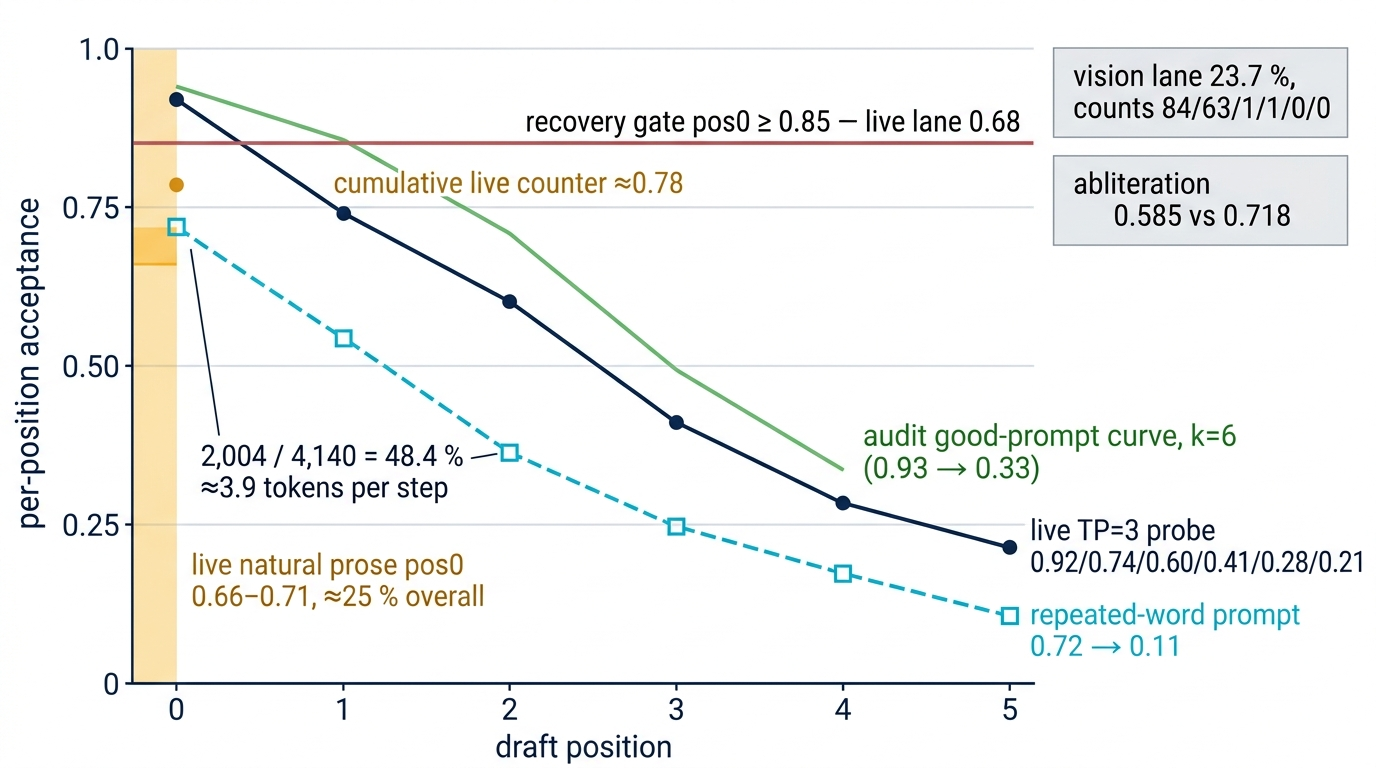
\includegraphics[width=\textwidth]{figures/ch08-acceptance-curves.png}
\caption{The same drafter, measured four ways. Audit-style numbered-word
probes hold pos0 at or above 0.90 with the normal DSpark collapse to about
0.33 by position 4; a live TP=3 probe accepted 2{,}004 of 4{,}140 drafted
tokens (48.4\,\%, $\approx$3.9 tokens per step); live natural prose sits at
pos0 0.66--0.71 with roughly 25\,\% overall against a cumulative live counter
of $\approx$0.78; and a degenerate repeated-word prompt collapses the drafter
from 0.72 to 0.11, reading as a fake $\approx$45 \tokspersec{} regression.
During the September campaign a recovery gate demanding pos0 $\ge 0.85$
failed against a live lane at 0.68 --- a pre-existing live-versus-audit gap,
not a regression. Never quote an acceptance number without its probe family.}
\label{fig:specdecode-probe-families}
\end{figure}

\subsection{Measuring it correctly}

The instrument is \repofile{scripts/spec-acceptance.py} (104 lines), run as
phase 2 of every serving audit: snapshot the
\code{vllm:spec_decode_*} counters, drive a short controlled burst, snapshot
again, and report \emph{window deltas} --- overall acceptance
$= \Delta\text{\texttt{accepted}}/\Delta\text{\texttt{drafted}}$,
per-position rate
$= \Delta\text{\texttt{per\_pos}}[i]/\Delta\text{\texttt{drafts}}$, tokens
per step
$= \Delta\text{\texttt{accepted}}/\Delta\text{\texttt{drafts}} + 1$.
Reporting the second
snapshot alone would print the container's lifetime totals, which describe
nothing about the burst just measured.

The instrument itself carries a lesson in metrics-parsing humility.

\begin{hbwarstory}
\textbf{The curve that never printed.} Until PR \ghissue{91}, the
per-position curve had \emph{never printed anything}: the parser split the
Prometheus line on \code{position=} and then on a comma, assuming another
label followed. But the pinned image emits \code{position} as the
\emph{last} label, so the parse yielded the fragment \texttt{0"\}~40263.0},
\code{int()} raised, and a bare \code{except} swallowed every position. The
fix anchors a regex directly on the \code{position} label's quoted digits,
reads \code{drafts_total} so counts become rates, and requires the
\code{_total} suffix on every counter match --- because the sibling \code{_created}
gauge carries a Unix timestamp that a naive prefix match happily reads as a
counter. The instrument now has its own regression suite
(\repofile{scripts/test-spec-acceptance.py}), including the case where spec
decode is off and the case where counters vanish between snapshots.
\end{hbwarstory}

\section{Choosing \texorpdfstring{$k$}{k}}
\label{sec:specdecode-choosing-k}

The tail of \Cref{fig:specdecode-curve} is an economic argument: a position
accepting 0.15 of its drafts adds a query row to every verify pass for
almost no accepted tokens. Acting on that argument, however, first required
deleting a rule. It is worth holding onto what $k$ actually moves: the
positions drafted, the query rows every verify pass carries, and the
CUDA-graph shapes the decode step must dispatch to --- and only the first of
those appears in an acceptance curve.

\subsection{The divisibility rule, and why DSpark is exempt}

Stock vLLM's \code{SpeculativeConfig.__post_init__} rejects any
\code{num_speculative_tokens > n_predict} not divisible by \code{n_predict}
(``Ensure divisibility for MTP module reuse''). That rule is correct for
stock MTP, which re-runs one draft layer per token. It is meaningless for
DSpark: the \code{mtp.0}--\code{mtp.2} stages are stacked into one backbone that
predicts the whole \code{dspark_block_size} block in a single pass, so the
stage count says nothing about draftable tokens. The rule's practical damage:
Vision-Exp ships \code{num_nextn_predict_layers=3} with
\code{dspark_block_size=5}, and the forced multiple-of-3 pushed the recipe to
$k{=}6$ --- one more noise query than the block was trained with. The
checkpoint's own \repofile{inference/model.py} \code{DSparkBlock} drafts
exactly $\gamma{=}5$ tokens; $k{=}5$ is the trained shape.

The unlock, \repofile{patches/hotfix-vllm-dspark-block-k.py}, is the
strictest patcher family in the repository (\Cref{ch:patches}): SHA-pinned
whole-file identity on \repofile{config/speculative.py}, pinned vLLM version
string, and a one-condition change --- \code{self.method != "dspark"}
prepended to the divisibility check. Gated by
\envvar{DSPARK_ENABLE_DSPARK_BLOCK_K=1}, paired with
\envvar{MTP_NUM_TOKENS=5}, fail-closed on any byte drift.

\begin{table}[htbp]
\centering\small
\caption{Vision-Exp, $k{=}5$ (block-$k$ unlock) vs.\ $k{=}6$
(divisibility-forced), same machine, 2026-09-03.}
\label{tab:specdecode-blockk}
\begin{tabular}{lccc}
\toprule
Metric & $k{=}5$ & $k{=}6$ & Delta \\
\midrule
Greedy decode, 8K ctx (\tokspersec{}) & 56.6 & 55.3 & $+2$\,\% \\
Greedy decode, 32K ctx (\tokspersec{}) & 56.6 & 53.6 & $+6$\,\% \\
Temp 0.6 decode (\tokspersec{}) & 49.9--56.9 & 48.6--53.1 & $+3$--$7$\,\% \\
Single-stream mini-bench (\tokspersec{}) & 56--64 & 51--55 & up to $+10$\,\% \\
Concurrency-4 aggregate (\tokspersec{}) & 110 & 106--111 & unchanged \\
TTFT & \multicolumn{2}{c}{unchanged} & --- \\
\bottomrule
\end{tabular}
\end{table}

The interpretation matters: per-position acceptance measured the same at
either $k$ (0.88 / 0.74 / 0.53 / 0.36 / 0.24), so the 2--10\,\% win is not better
drafting --- it is the cheaper step. Position 5 was accepting 0.15 of its
drafts while adding a query row to every verify pass; deleting it is nearly
pure profit at low concurrency and washes out at $c{=}4$ where the batch is
already amortizing the stream.

\subsection{The capture-size coupling}

$k$ is not a free-standing knob. The uniform decode step processes
\code{MAX_NUM_SEQS} $\times (k{+}1)$ tokens, and the CUDA-graph capture list
must include that shape, rounded up to a multiple of 8 (40 at
$6\times 6$ rows for $k{=}5$; 48 for $k{=}6$). The TP=2 lane shipped for
weeks violating exactly this coupling --- the literal boot log line was
``Truncating max\_cudagraph\_capture\_size to 40'' --- so every
full-concurrency step ran eager. \Cref{ch:perf} tells the full
predict--fix--verify arc, measured cost included. When you change $k$,
recompute the capture size; \repofile{scripts/validate-dspark-config.sh}
prints the unrounded product for exactly this reason.

Finally, the official model cards pair \code{num_speculative_tokens=7} with
\emph{greedy} draft sampling (issue \ghissue{84}). This recipe's compose
defaults to \code{probabilistic} at the trained block width, and its greedy
A/B measured a tie on this hardware. Both are legitimate operating points;
what is not legitimate is changing draft sampling and $k$ together and
attributing the delta to either alone.

\section{Tensor parallelism and the draft loop}
\label{sec:specdecode-tp}

Choosing $k$ prices the draft loop in query rows; tensor parallelism prices
the same loop in network round-trips.

\subsection{Twelve serialized collectives}

The Anemll image shards the Markov head with TP: \code{markov_w1} is a
\code{VocabParallelEmbedding} (all-reduce per lookup) and \code{markov_w2} a
\code{ParallelLMHead} whose logits route through the vocab-parallel
\code{LogitsProcessor} (all-gather). The draft block is sampled
left-to-right, so at $k{=}6$ the loop pays 2 collectives $\times$ 6 steps =
\textbf{12 serialized collectives per decode step} --- serialized because
each position's Markov bias depends on the token chosen at the previous one.
\Cref{ch:perf}'s collectives census prices the step's full collective
budget; what matters here is that the Markov dozen are the only entries in
it that cannot overlap with anything. Both Markov matrices are 66\,MB ---
replication is essentially free --- and the upstream source even carries a
\code{TODO(ben): profile ... replicate or TP-shard} comment.

\subsection{An honest negative result}

The obvious fix exists as
\repofile{patches/hotfix-dsv4-replicate-markov-head.py}:
\code{markov_w1} becomes a plain \code{nn.Embedding}, \code{markov_w2} a
\code{ReplicatedLinear}, and \code{bias()} computes locally, skipping the
\code{LogitsProcessor} all-gather entirely --- the Anemll-image equivalent
of the Stage-C overlay flag
\envvar{VLLM_DSPARK_REPLICATE_MARKOV_W1}. The
patch is correct: the A/B showed acceptance unchanged, proving the replicated
math matches the sharded math. And yet the verdict was \textbf{OFF}: no
measurable $c{=}1$ gain (the predicted 0.5--1.5\,ms is under the lane's
$\pm$10 \tokspersec{} prompt-draw noise), and the $c{=}6$ aggregate ran 122 vs.\
148 \tokspersec{} against the same-day baseline. The repository keeps the patch, its
tests, and the negative verdict side by side.

\begin{hblesson}
A first-principles estimate of 1--3\,\% is a reason to \emph{try} a patch,
not to ship it. This lane's single-stream throughput swings
$\approx$48--76 \tokspersec{} with the prompt drawn; three trials cannot resolve a
1--3\,\% knob. The campaign's rule --- eight pooled trials, same-day
baseline, host-memory gate before measuring --- exists precisely so that a
correct-but-unhelpful patch gets an honest OFF instead of a flattering
anecdote. Correctness A/Bs (acceptance unchanged) and performance A/Bs
(aggregate down) answer different questions; run both.
\end{hblesson}

\subsection{Variable-length drafting: the confidence schedulers}

The Stage-C overlay carries machinery the pinned production lane does not yet
enable: per-position confidence heads
(\code{sigmoid(proj([dense || markov_embed]))}) feeding a draft-length
scheduler behind \envvar{VLLM_DSPARK_CONFIDENCE_SCHEDULER}. The support
library (\repofile{recipe/overlay/vllm/v1/spec_decode/dspark.py}) turns
conditional per-token confidences into prefix survival probabilities and
truncates the draft \emph{non-anticipatingly} --- position $n$ admitted
using only confidences $\le n$, preserving rejection-sampling compatibility.
A hardware-aware variant scores candidate prefix schedules
against a profiled steps-per-second curve. This is the principled version of
the block-$k$ observation: position 5 at 0.15 acceptance should usually not
be drafted, and a confidence head can make that call per request per step.

Speculation stops reading as an accelerator bolted onto decode once the
weight stream is the entire cost. On this hardware the drafter \emph{is} the
decode architecture, and $k$, the ring buffers, the Markov collectives and
the CUDA-graph capture list are one coupled design rather than a knob with
side effects --- change $k$ and you change the query rows in every verify
pass and the shapes the step must dispatch to. Acceptance changed character
too: it is not a constant of the model but a joint measurement of drafter,
prompt family and instrument, which is why the same engine honestly reports
0.93 at position 0 and 0.68, and why a gate written against the wrong number
nearly manufactured a regression that was never there.

\FloatBarrier
\section*{Takeaways}

\begin{itemize}
  \item On bandwidth-bound hardware, one verify pass amortizes a
    16--17\,GB weight stream over $k{+}1$ token positions; at
    $\approx$4 accepted tokens per step this is the difference between
    $\sim$15 and the August-published 62--83 \tokspersec{} band on TP=2.
    Acceptance rate is the lever,
    and DSpark pulls it by drafting a whole $\gamma{=}5$ block in one
    non-causal pass (anchor + noise queries), sampling left-to-right through
    a rank-256 Markov bias, and keeping its only cross-step state in
    per-attention-module ring buffers \emph{outside} vLLM's paged KV.
  \item That private state is what breaks under concurrency. Any stateful
    component indexed by batch row will be corrupted by a condensing
    scheduler, so key it by request identity (Patch~1) with an
    identity-permutation fast path that keeps single-stream behavior
    byte-exact --- and remember that raggedness comes from chunked prefill,
    not from rejection: Patch~2 made the context path ragged via
    \code{query_start_loc}, and Patch~2b, found by a GSM8K eval rather than a
    benchmark, decoupled ragged detection from the rejection tensor. Run
    quality evals under concurrency; they reach code paths benchmarks never
    do.
  \item Acceptance is strongly prompt-dependent --- pos0 $\ge 0.90$ on
    numbered-word probes vs.\ 0.66--0.71 on live natural prose, with
    repeated-word prompts collapsing the drafter entirely --- so never gate
    on a number without knowing which probe family produced it. Measure it as
    counter \emph{deltas} over a controlled burst, never lifetime totals;
    anchor on \code{_total} (the \code{_created} sibling is a timestamp); and
    remember the curve that ``always printed nothing'' until PR \ghissue{91}.
    Instruments deserve regression tests.
  \item The MTP divisibility rule does not apply to stacked-stage drafters;
    running the trained block width ($k{=}5$) bought a measured 2--10\,\% by
    making the step cheaper, not the drafts better. Recompute
    \code{MAX_NUM_SEQS} $\times (k{+}1)$ capture sizes whenever $k$ changes.
  \item TP puts 12 serialized collectives inside the Markov sampling loop;
    replicating the 66\,MB head is correct but measured no win on this
    fabric --- keep honest negative results next to the patch they judge.
\end{itemize}

\chaptertransition{Acceptance multiplies the tokens a step produces, but the
step itself is priced in bytes and network round-trips --- and this chapter
kept spilling into that ledger. Twelve serialized collectives inside the
Markov loop, a capture list that must be recomputed whenever $k$ moves, a
replicated head that was provably correct and still lost throughput: none of
those verdicts can be read without the whole equation written down, stating
what a decode step must stream, what it must synchronize, and what remains
that no configuration reaches. The next chapter writes it, then spends two
one-knob-per-boot campaigns testing every lever against it. Its sharpest
result is the one nobody wanted: a third node cut the bytes each rank streams
to roughly 11.5\,GB and the model priced the step at 48\,ms --- and the
measured decode rate did not move at all.}
